\graphicspath{{../images/intro/}}
\chapter{Постановка задачи и обзор существующих методов}
\todo{существенно меняла текст начиная с раздела 1.2}
\section{Белки. Основные определения}
% - что такое белки
% - из чего состоят
% - что такое поверхность белка
% - информация о вторичной структуре 
%(мб сказать что такое вторичная структура белка?  вынести во введение или первую главу)
%Зачастую являясь результатом несинонимичной замены одного нуклеотида, точечная мутация одной аминокислоты может приводить к масштабным последствиям: так, например,
%\todo{дописать}

%\todo {вообще здесь должно быть не про точечные мутации, а какие-то общие слова. Блаблабла, дизайн лекарств, блаблабла. и при чем тут белки.}
\subsection{Белки как основа живой материи}
\textbf{Первичная структура} белка задается последовательностью (\textbf{цепочкой}) аминокислот:

\resizebox{0.9\textwidth}{!}{
%\input{aa3_5.tex}
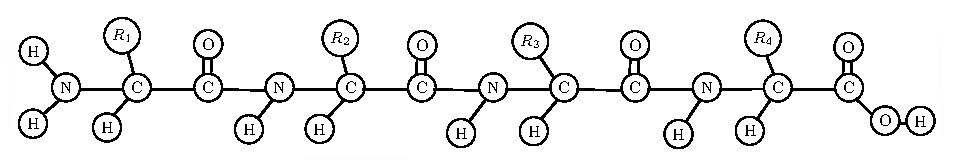
\includegraphics{aa3_1.eps}
}

\textbf{Вторичная структура} задается укладкой цепочки аминокислот в пространственные структуры, \textbf{третичная структура} - расположением этих структур в пространстве в случае, когда белок содержит только одну цепь.

Когда белок состоит из нескольких цепей, говорят о его \textbf{четвертичной структуре}.

\subsection{Белки и энергия}
С точки зрения химии, разным видам структуры соответствуют разные виды химических связей и электростатических взаимодействий.

Когда мы рассматриваем несколько цепочек в составе одного белка или несколько белков, образующих комплекс, мы говорим о \textbf{белок-белковом взаимодействии}.

\textbf{Интерфейс} такого взаимодействия -- это участки \textbf{поверхности} белков, непосредственно контактирующие между собой.

Свободная энергия связи, обозначаемая \ddG, определена как разность $\vartriangle\!G_{mut} - \vartriangle\!G_{wt}$ , где $\vartriangle\!G_{wt}$ и $\vartriangle\!G_{mut}$ -- изменения свободной энергии Гиббса для немодифицированного белка (как еще перевести wild-type?? чтоб не в лоб) и его подвергнутой точечному мутагенезу версии (alanine-mutated
protein).

\subsection{Поверхность белка как его энергетический фронт}
\subsection{Белок-белковое взаимодействие}
Рассмотрим белок, имеющий четвертичную структуру.

\textbf{Вопрос}: можно ли изменить что-то в его структуре, чтобы образующие его цепочки были лучше сцеплены между собой?

Пусть есть комплекс из двух белков (например, имунноглобулин и эпитоп).

\textbf{Вопрос 1}: можно ли изменить что-то в его структуре, чтобы усилить связь между компонентами комплекса?

\textbf{Вопрос 2}: насколько специфична одна из компонент комплекса?  Можно ли подобрать один из белков так, чтобы комплекс был более устойчивым? Насколько заменяема каждая из компонент?

Ответить нам поможет \textbf{аланиновое сканирование} (аланиновый мутагенез).
\newpage
\section{Аланиновое сканирование}
Аланиновое сканирование (ала-скан)~\cite{alascan2001} - метод для определения аминокислот в составе белка, играющих важную роль в сохранении его функций, стабильности или формы.

Первоначальная идея метода очень проста: заменить одну из аминокислот в цепочке на любую другую и посмотреть, повлияет ли такое точечное изменение (точечный мутагенез) на энергию комплекса, приведет ли это к усилению или ослаблению взаимодействия между цепочками белков. 

Но как выбирать аминокислоту, на которую проводить замену? Всегда ли стоит перебирать все аминокислоты в одной и той же позиции в цепочке?

Экспериментально было показано~\cite{alascan2001}, что достаточно заменить аминокислоту на аланин, чтобы понять, является ли она энергетически значимой при оценке взаимодействия цепочек, или нет. А затем, если изменение энергии комплекса \ddG\,  оказывается существенным, перебрать все оставшиеся аминокислоты в данной позиции и определить, какая замена является экстремальной.

Понять, почему для точечной мутации выбирают именно аланин, может помочь следующий рисунок, на котором в центре изображена химическая формула аланина, окруженная формулами других аминокислот (отличающиеся фрагменты радикалов аминокислот изображены красным цветом):

\begin{center}
 \resizebox{0.4\textheight}{!}{
 \ttfamily
 \footnotesize
 \aapicture
 }
\end{center}

Как видим, аланин -- аминокислота с коротким радикалом. Она относительно легкая, химически нейтральная. 

%\begin{wrapfigure}{RT}{0.3\textwidth}
%\resizebox{0.2\textwidth}{!}{
%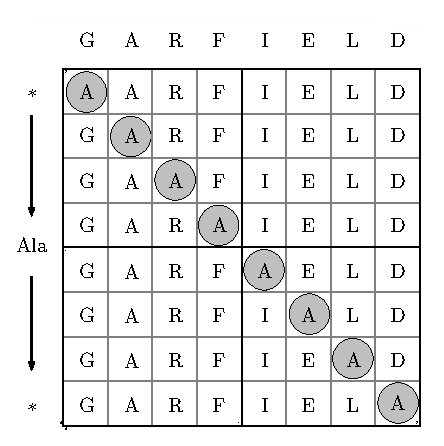
\includegraphics{ala_scan.eps}
%}
%\end{wrapfigure}

\subsection{Аланиновое сканирование in vitro/in vivo}
Первоначально аланиновое сканирование появилось как лабораторный, химический метод (in vitro/in vivo), с вытекающими отсюда свойствами:
\begin{itemize}
\item Большое пространство поиска: для того, чтобы определить энергетически значимые аминокислоты, требовалось проверить все.
\item Сложность синтеза библиотек: в каждом индивидуальном случае необходимо выбрать метод для синтеза, получить и разделить образцы с точечными мутациями в каждой из позиций цепочки. В отдельных случаях необходимо проводить рефолдинг полученных точечно-модифицированных белков.
\item Как следствие, высокая стоимость - как в денежном, так и во временном эквиваленте.
\end{itemize}

Создание библиотеки белков с точечными мутациями in vivo позволяет упростить получение модифицированных олигомеров, но оно доступно для ограниченного числа белков ~\cite{alascan2001}.

У экспериментального аланинового  сканирования есть один существенный ,,плюс'' -- оно позволяет выявить  аминокислоты, которые существенно влияют на функцию, стабильность или форму белка в клетке и оценить это это влияние с небольшой погрешностью. Причем результат такого эксперимента будет близок к тому, что произойдет в клетке. 

Чтобы сократить затраты на аланиновое сканирование в лаборатории, применяют теоретическое, компьютерное моделирование аланинового сканирования, в данной работе обозначенное как ala-scan in silico, в противовес экспериментальному лабораторному аланиновому сканированию. Обычно его используют для выбора потенциально важных аминокислот, но, разумеется, результаты проверяют в лаборатории, создавая экспериментальную библиотеку образцов с мутациями уже не по всем позициям, а только по выбранным in silico, сокращая тем самым стоимость эксперимента.

Посмотрим, каким образом происходит аланиновое сканирование in silico.
%уточнить цифру \newpage
\subsection{Аланиновое сканирование in silico: решаемые задачи и границы применимости}

Компьютерное моделирование аланинового сканирования позволяет удешевить разработку лекарственных средств: с его помощью решают различные задачи, возникающие при разработке современных, высокотехнологичных лекарств. С помощью модификации всего одной аминокислоты можно оценить специфичность разрабатываемого лекарства, синтезировать новый, не запатентованный белковый препарат, не отличающийся по эффективности от уже запатентованных, или, например, убедиться в том, что разрабатываемый препарат не взаимодействует с важными функциональными элементами клетки. 


Если при экспериментальном аланиновом сканировании можно относительно точно оценить, насколько изменилась свободная энергия комплекса после замены одной аминокислоты, то при компьютерном моделировании приходится применять различные методы для грубой оценки этого изменения. Еще одна задача, которую необходимо решать - правильно (в смысле реалистичности происходящего изменения) проводить рефолдинг -- пересборку олигомера после точечной мутации.

Так, например, для уточнения структуры, которую примет цепочка с точечной мутацией и исследуемый комплекс в целом, используются различные методы -- от приближенных, но универсальных, таких как метод Монте-Карло на решетке \cite{monte_carlo}, до точных, но специфичных для конкретного белка, таких как моделирование с помощью методов молекулярной динамики.

Основная цель этого действа -- достоверно оценить, насколько и в какую сторону измененится изменение свободной энергии Гиббса \ddG комплекса при внесении точечной мутации в одну из цепочек:
$$
\Delta\Delta G_{bind} = (\Delta G_{M complex} - \Delta G_{M_A} - \Delta G_{M_B}) - (\Delta G_{WT complex} - \Delta G_{WT_A} - \Delta G_{WT_B})
$$

В данной работе используется протокол аланинового сканирования из пакета rosetta, с немодифицированной функцией свободной энергии. Как было показано в работе \cite{kortemme2002}, такая функция  эффективно предсказывает изменение энергии комплекса в случаях, когда вода исключена из рассмотрения.

Детали реализации протокола не приводятся, поскольку их рассмотрение не является основной целью данной работы.
%\todo{сказать, что в данной работе используется протокол из rosetta (мб привести картинку про реальную ddG и in silico функцию изменения энергии), сцепленность цепочек оценивается в смысле изменения энергии, применяемый в протоколе метод монте-карло лежит за пределами работы (кроме того, является относительно хорошо изученным, в ходе работы никакие модификации в сам метод или функцию оценки ddG не вносились), поэтому не приводится. }





%\newpage
\section{Стандартные методы выбора аминокислот для аланинового сканирования in silico}

Как правило, при компьютерном моделировании аланинового сканирования проводят предварительную фильтрацию аминокислот, после которой проводится сканирование. 

Для фильтрации используются два основных метода~\cite{hotspots2012rev}:
\begin{itemize}
\item отсечка по расстоянию;

\item выбор по гомологии.
\end{itemize}

Оценим эффективость каждого из этих подходов.

\subsection{Выбор аминокислот вблизи интерфейса взаимодействия с отсечкой по расстоянию}

Способ фильтрации аминокислот, при котором выбираются для последующей мутации только те из них, которые находятся вблизи интерфейса взаимодействия компонент исследуемого комплекса, в определенном смысле биологически обоснован. Во-первых,  консервативные в смысле эволюции белков аминокислоты являются таковыми потому, что вносят важный вклад в сохранение функций, стабильности или формы белка \cite{toadd}. Они же часто оказываются в области интерфейса взаимодействия белков. Во-вторых, энергетически важные аминокислоты обычно специфичны по отношению к взаимодействующему комплексу белков \cite{toadd1}, так же, как и интерфейс такого взаимодействия, поэтому эти понятия часто не различают.

Способ выбора аминокислот с  отсечкой по расстоянию от интерфейса взаимодействия ~\cite{kortemme2004} -- универсален, он может использоваться и при дизайне de novo, то есть в ситуациях, когда белок синтезируется впервые, экспериментальное аланиновое сканирование эволюционно близких к нему белков ранее не проводилось. 

Как правило, в качестве величины отсечки берут величину порядка  4-8 \AA{}. В  Rosetta Alascan Protocol~\cite{kortemme2004} используется усложнение: дополнительно рассматриваются аминокислоты, $\beta$-углерод которых после формирования комплекса в шаре определенного фиксированного радиуса содержит существенно больше атомов $\beta$-углерода, чем содержал до этого.

%\newpage
Чтобы показать, почему такой подход не всегда эффективен, проведем эксперимент in silico:
\begin{enumerate}
\item Рассмотрим базу данных с информацией о результатах эспериментов по аланиновому сканированию белков ASEdb~\cite{asedb2001}. Найдем объекты с корректными ссылками на записи в Protein Data Bank ~\cite{rcsb}.
\item Среди всех таких объектов найдем те, в которых есть аминокислоты, мутация которых приводит к существенному изменению свободной энергии комплекса ($\geq 1$ ккал/моль)
\item Посмотрим, всегда ли такие аминокислоты удалены от интерфейса в пределах стандартно используемой отсечки (в качестве примера возьмем расстояние, не превышающее 8 \AA{}).
\end{enumerate}

Результат работы скрипта для PyMOL, отображающего результаты этого эксперимента, показан на следующем рисунке: 

\resizebox{0.8\textwidth}{!}{
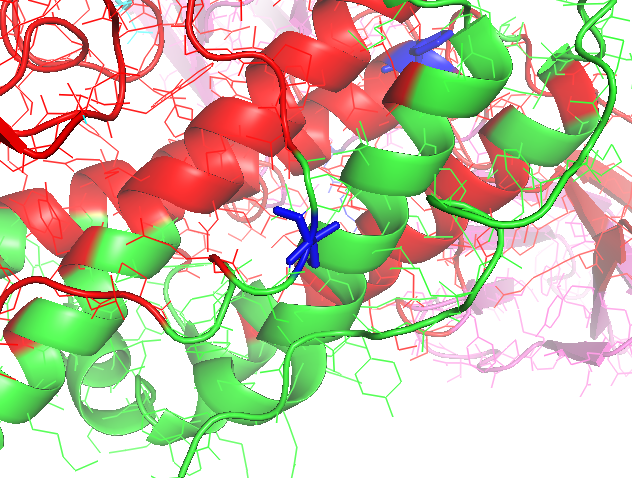
\includegraphics{image7.png}
}

На приведенном скриншоте красным цветом ,,окрашены'' аминокислоты одной из цепочек, атомы которых удалены от атомов парной цепочки, образующей исследуемый комплекс, не более, чем на 8 \AA{}. синим цветом ,,окрашены'' аминокислоты, точечное изменение которых приводит к существенному изменению свободной энергии комплекса. 

Как видим, метод фильтрации аминокислот с отсечкой по расстоянию от интерфейса взаимодействия белков иногда упускает из рассмотрения аминокислоты, которые влияют на взаимодействие пары олигомеров, но при этом удалены от области интерфейса.

Такие аминокислоты, например, могут находиться в глубине карманов на поверхности одного из белков и, тем не менее, оказывать существенное влияние на стабильность белкового комплекса в целом \cite{pockets2004}.
%\newpage
\subsection{Поиск по гомологии}

%: аминокислоты отбираются исходя из имеющихся экспериментальных результатов аланинового сканирования, проводившихся на близких (в эволюционном смысле) последовательностях.

Для эффективного поиска по гомологии необходимо иметь базу близких (ортологичных) структур, точную и содержащую всю информацию по результатам аланинового сканирования.

Метод должен учитывать как данные о последовательности аминокислот в белках, так и каким-либо образом эксплуатировать пространственную структуру. В качестве примеров методов, учитывающих и то, и другое, можно привести ~\cite{hhm_svm}.

%Проводятся попытки классификации участков, 
%здесь можно ссылку на диссертацию студентки Фришмана

После того, как в лабораторной практике стали применяться различные техники эспериментального аланинового сканирования, появились и базы данных с его результатами ~\cite{asedb2001, bid2003}, но они фрагментированы, не всегда полны, разнородны (вероятно, это связано с тем, что данные собираются из разных источников и статей). Кроме того, данных в них не так много -- в силу приведенных выше свойств экспериментального точечного мутагенеза в лаборатории.

Например, если Protein Data Bank содержит информацию о большом количестве структур, с примерно одним и тем же форматом данных, то asedb представляет собой базу данных mysql и содержит информацию о 101 структуре, а BID доступна в виде набора wiki-страниц с информацией о конкретных белках или парах взаимодействующих цепочек.

Единообразные и относительно сгруппированные данные представлены в наборе данных  \cite{kortemme_alascan_datasets}, который изначально был собран из разных источников для оценки работы компьютерного протокола аланинового сканирования в составе пакета Rosetta \cite{kortemme2002, kortemme2004}. 